
%%%%%%%%%%%%%%%%%%%% file cmmr12_template.tex %%%%%%%%%%%%%%%%%%%%%
%
% This is the LaTeX source for the instructions to authors using
% the LaTeX document class 'llncs.cls' for contributions to
% the Lecture Notes in Computer Sciences series.
% http://www.springer.com/lncs       Springer Heidelberg 2006/05/04
%
% It may be used as a template for your own input - copy it
% to a new file with a new name and use it as the basis
% for your article.
%
% NB: the document class 'llncs' has its own and detailed documentation, see
% ftp://ftp.springer.de/data/pubftp/pub/tex/latex/llncs/latex2e/llncsdoc.pdf
%
%%%%%%%%%%%%%%%%%%%%%%%%%%%%%%%%%%%%%%%%%%%%%%%%%%%%%%%%%%%%%%%%%%%


\documentclass[runningheads,a4paper]{llncs}

\usepackage{amssymb}
\setcounter{tocdepth}{3}
\usepackage{graphicx}
\usepackage{url}
\newcommand{\keywords}[1]{\par\addvspace\baselineskip
\noindent\keywordname\enspace\ignorespaces#1}

\pagestyle{headings}

\begin{document}

\mainmatter  % start of an individual contribution

% first the title is needed
\title{From Faust to WebAudio: Compiling Faust to JavaScript using Emscripten to make noise in the browser.}

% a short form should be given in case it is too long for the running head
\titlerunning{From Faust to WebAudio}

% the name(s) of the author(s) follow(s) next
%
% NB: Chinese authors should write their first names(s) in front of
% their surnames. This ensures that the names appear correctly in
% the running heads and the author index.
%
\author{Myles Borins \thanks{Julius O. Smith, Stéphane Letz, Yann Orley, and Colin Clark}}
%
% if the names of the authors are too long for the running head, please use the format: AuthorA et al.
\authorrunning{Myles Borins}

% the affiliations are given next; don't give your e-mail address
% unless you accept that it will be published
\institute{Center For Computer Research in Music and Acoustics\\ \email{mborins@ccrma.stanford.edu}}

%
% NB: a more complex sample for affiliations and the mapping to the
% corresponding authors can be found in the file "llncs.dem"
% (search for the string "\mainmatter" where a contribution starts).
% "llncs.dem" accompanies the document class "llncs.cls".
%


\maketitle


\begin{abstract}
% The abstract should summarize the contents of the paper and should
% contain at least 70 and at most 150 words. It should be written using the
% \emph{abstract} environment.
The WebAudio API is a platform for doing audio synthesis in the browser.  Currently it has a number of natively compiled audio nodes capable of doing fairly advanced synthesis.  One of the available node the "JavaScriptNode" allows individuals the ability to create their own custom unit generators in pure JavaScript. While a number of people have been writing custom nodes, they are rewriting code that has been perfected multiple times in various languages. The Faust project, developed at Grame CNCM, offers a unique solution to this problem.  Faust consists of both a language and a compiler, allowing individuals to deploy a signal processor to various architectures including Max/MSP, supercollider, and core-audio.  This paper examines a technology stack that allows for Faust to be compiled to highly optimized JavaScript unit generators that synthesize sound using the web audio api.  


\keywords{Faust, Flocking, WAAX, JavaScript, asm.js, emscripten}
\end{abstract}


\section{Introduction}

The WebAudio API, released in 2011, is "a high-level JavaScript API for processing and synthesizing audio in web applications."\footnote{\url{https://dvcs.w3.org/hg/audio/raw-file/tip/webaudio/specification.html}}  Currently there are a number of natively compiled audio nodes within the API capable of doing fairly advanced synthesis. One of the available node the "JavaScriptNode" allows individuals the ability to create their own custom unit generators in pure JavaScript. 

While the concept of making interactive sound synthesis environments in the browser is quite exciting, there are two primary factors stopping individuals from investing time into the web audio platform; There has not yet been enough Signal Processing related JavaScript code written yet, and some signal processing concepts prove difficult to implement efficiently in a loosely typed language with no memory management.

\subsection{WAAX and Flocking}

There are a number of projects that are in development abstracting over top of the WebAudio API in order to extend its capabilities by creating more complicated unit generators and a more intuitive syntax.  Projects such as WAAX (Web Audio API eXtension)\footnote{\url{https://github.com/hoch/waax}} by Hongchan Choi use the native nodes only in order to ensure optimum efficiency.\cite{waax}

The Flocking audio synthesis toolkit\footnote{\url{http://flockingjs.org/}} by Colin Clark offers a unique declarative model for doing signal processing within the browser.  Unlike WAAX, Flocking has opted to use the "JavaScriptNode" for all unit generators giving users access to a number of signal processing algorithms that can not be achieved using only native nodes.

WAAX and Flocking offer individuals two very different approaches to web audio. WAAX offers efficiency, whereas Flocking offers bleeding edge unit generators.  That being said both projects suffer from the same problem, a lack of man hours.  There are only so many individuals who have the time and domain specific knowledge necessary to write new unit generators.

\subsection{Faust}
The Faust project offers a unique solution to this problem; rather than write code, generate it.  Faust, developed at Grame CNCM,"is a programming language that provides a purely functional approach to signal processing while offering a high level of performance." \cite{orlarey:09c}  The project is both a language and a compiler, offering the ability to write code once and deploy to many different signal processing environments.



This section will continue to describe the current state of Faust -> Web audio compilation, specifically the problems with the current process which is inline with the above mentioned problems (efficiency, language limitations).  It will then introduce Emscripten\footnote{\url{https://github.com/kripken/emscripten}} a cross compiling tool designed to compile C/C++ into efficient asm.js code.  Asm.js \footnote{\url{http://asmjs.org/}} will also be introduced as a subset of javascript that "provides a model closer to C/C++ by eliminating dynamic type guards, boxed values, and garbage collection."\cite{asm-js}.

\section{A Simple Approach}

A first approach to automating the compilation process from Faust to Flocking involves manually implementing each step. The Faust code needs to be compiled to C++, from there it needs to compiled to LLVM bytecode by either Faust2 or emscripten.  Once compiled to bytecode emscripten needs to be used to compile to asm.js.  The asm.js needs to have binding functions written to get access to the compiled code within the javascript environment.  These functions then need to be hooked into the web audio api.  Finally bindings need to be written between these functions and the Flocking toolkit.

\subsubsection{Making Noise:}

A first test was to attempt to compile the example noise.dsp that comes shipped with Faust.  Noise was chosen as it is currently broken in the current iteration of Faust -> Web Audio Api.  Due to the integer specific calculations required for the Faust implementation of noise, a satisfactory result was unable to be accomplished using the current system.

The below sections will be used to describe the process used to manually implement noise in the browser starting from a faust dsp file, and ending with a working Flocking Synthdef.

\subsection{Faust}

The noise unit generator starts as a Faust dsp file.  It's code is fairly straight forward.

\begin{verbatim}
random  = +(12345)~*(1103515245);
noise   = random/2147483647.0;
process = noise * vslider("Volume[style:knob]", 0, 0, 1, 0.1);
\end{verbatim}

Faust is able to compile this to optimized C++ out of the box.  Currently if you compile without selecting an architecture file then a number of things are missing from the C++, specifically the include files as well as the definition for the dsp object (which it appears is dependent on audio architecture specified). Is it possible to get the appropriate headers and class definitions compiled into the C++ without selecting an architecture file?  If not what type of information should be generated for the web audio architecture

Another thing worth exploring is wether or not the faust code should be compiled to LLVM bytecode rather than C++, this will require a conversation with Stephane and Yann to figure out.

\subsection{Emscripten \& asm.js}

Once you have the optimized C++ properly compiled (or llvm bytecode) it can then be compiled to asm.js using Emscripten.  There are a handful of features of C++ that are not supported by Emscripten included vectorized optimizations, so it might necessary to do a number of tests before being able to properly compile asm.js

\subsection{Web Audio Api}

Once the asm.js code has been compiled a JavaScript file needs to be written in order to both break out the functionality of the code into JavaScript functions.  As well, the correct context for generating audio in the browser needs to be set up within the web audio api, connecting the generated data from the Faust generated functions to the correct web audio api functions in order to generate sound.

\subsection{Flocking}

Once the web audio unit generators have been properly implemented, the final stage involves wrapping the web audio unit generator to be controlled by the Flocking toolkit.  This process may or may not be trivial depending on how the above web audio code ends up being generated.

\section{Automation}

All the above steps should be able to be automated, if time permits this section will examine how an architecture file can be written in order to compile any faust dsp file to the web audio api and Flocking.

\section{Results}

This will be a quick look at the resulting generated signal, if it is indeed an accurate instance of noise, and how the signal compares to faust compiled noise generated in other signal processing environments.  It may also be worth examining performance benchmarks, if a good model can be found to do so.

\section{Looking Forward}

This section will discuss current implementations of the above used technologies, and what type of improvements can be expected over time.  Asm.js is getting both AOT and JIT optimizations built directly in the browser, currently only in Firefox, but when implemented in Chrome there will be some great improvements to efficiency.  

Web audio api is currently only supported in Chrome, but work has begun to implement it in firefox.  This creates an interesting problem where the most efficient browser to run the compiled code is unable to actually do anything with it due to not supporting web audio api yet.

Talk about How other web based frameworks can bootstrap on this idea in order to get use of the various unit generators that can be generated from this process.  Once the compiled code is hooked into the web-audio api bindings can be written for any framework.

Finally discuss a conclusion about findings of the project

\section{Code Repository}

The entire source code can be found online on GitHub at:
\\
\url{https://github.com/TheAlphaNerd/faust2webaudio}

\begin{thebibliography}{1}
	
    % \bibitem{orlarey:09c}
    % Y.~Orlarey, D.~Fober, and S.~Letz.
    %      \textsl{New Computational Paradigms for Computer Music},
    % \newblock 2009.

    \bibitem{waax}
    H.~Choi, J.Berger., ``WAAX: Web Audio API eXtension"
    \emph{Proceedings of the Thirteenth New Interfaces for Musical Expression Conference}, 2013.
    
	
    \bibitem{orlarey:09c} Y.~Orlarey, D.~Fober, and S.~Letz., ``FAUST : an Efficient Functional Approach to DSP Programming,"
    \emph{New Computational Paradigms for Computer Music}, pp. 65-96, Editions DELATOUR FRANCE, 2009.

	\bibitem{asm-js}
	\textsl{asm.js - frequently asked questions.}
    \newblock \url{http://asmjs.org/faq.html.}
    
    
	
\end{thebibliography}

% \section{Paper Preparation}
% 
% Springer provides you with a complete integrated \LaTeX{} document class
% (\texttt{llncs.cls}) for multi-author books such as those in the LNCS
% series. Papers not complying with the LNCS style will be reformatted.
% This can lead to an increase in the overall number of pages. We would
% therefore urge you not to squash your paper.
% 
% Please always cancel any superfluous definitions that are
% not actually used in your text. If you do not, these may conflict with
% the definitions of the macro package, causing changes in the structure
% of the text and leading to numerous mistakes in the proofs.
% 
% If you wonder what \LaTeX{} is and where it can be obtained, see the
% ``\textit{LaTeX project site}'' (\url{http://www.latex-project.org})
% and especially the webpage ``\textit{How to get it}''
% (\url{http://www.latex-project.org/ftp.html}) respectively.
% 
% When you use \LaTeX\ together with our document class file,
% \texttt{llncs.cls},
% your text is typeset automatically in Computer Modern Roman (CM) fonts.
% Please do
% \emph{not} change the preset fonts. If you have to use fonts other
% than the preset fonts, kindly submit these with your files.
% 
% Please use the commands \verb+\label+ and \verb+\ref+ for
% cross-references and the commands \verb+\bibitem+ and \verb+\cite+ for
% references to the bibliography, to enable us to create hyperlinks at
% these places.
% 
% For preparing your figures electronically and integrating them into
% your source file we recommend using the standard \LaTeX{} \verb+graphics+ or
% \verb+graphicx+ package. These provide the \verb+\includegraphics+ command.
% In general, please refrain from using the \verb+\special+ command.
% 
% Remember to submit any further style files and
% fonts you have used together with your source files.
% 
% \subsubsection{Headings.}
% 
% Headings should be capitalized
% (i.e., nouns, verbs, and all other words
% except articles, prepositions, and conjunctions should be set with an
% initial capital) and should,
% with the exception of the title, be aligned to the left.
% Words joined by a hyphen are subject to a special rule. If the first
% word can stand alone, the second word should be capitalized.
% 
% Here are some examples of headings: ``Criteria to Disprove
% Context-Freeness of Collage Language", ``On Correcting the Intrusion of
% Tracing Non-deterministic Programs by Software", ``A User-Friendly and
% Extendable Data Distribution System", ``Multi-flip Networks:
% Parallelizing GenSAT", ``Self-determinations of Man".
% 
% \subsubsection{Lemmas, Propositions, and Theorems.}
% 
% The numbers accorded to lemmas, propositions, and theorems, etc. should
% appear in consecutive order, starting with Lemma 1, and not, for
% example, with Lemma 11.
% 
% \subsection{Figures}
% 
% For \LaTeX\ users, we recommend using the \emph{graphics} or \emph{graphicx}
% package and the \verb+\includegraphics+ command.
% 
% Please check that the lines in line drawings are not
% interrupted and are of a constant width. Grids and details within the
% figures must be clearly legible and may not be written one on top of
% the other. Line drawings should have a resolution of at least 800 dpi
% (preferably 1200 dpi). The lettering in figures should have a height of
% 2~mm (10-point type). Figures should be numbered and should have a
% caption which should always be positioned \emph{under} the figures, in
% contrast to the caption belonging to a table, which should always appear
% \emph{above} the table; this is simply achieved as matter of sequence in
% your source.
% 
% Please center the figures or your tabular material by using the \verb+\centering+
% declaration. Short captions are centered by default between the margins
% and typeset in 9-point type (Fig.~\ref{fig:example} shows an example).
% The distance between text and figure is preset to be about 8~mm, the
% distance between figure and caption about 6~mm.
% 
% To ensure that the reproduction of your illustrations is of a reasonable
% quality, we advise against the use of shading. The contrast should be as
% pronounced as possible.
% 
% If screenshots are necessary, please make sure that you are happy with
% the print quality before you send the files.
% \begin{figure}
% \centering
% 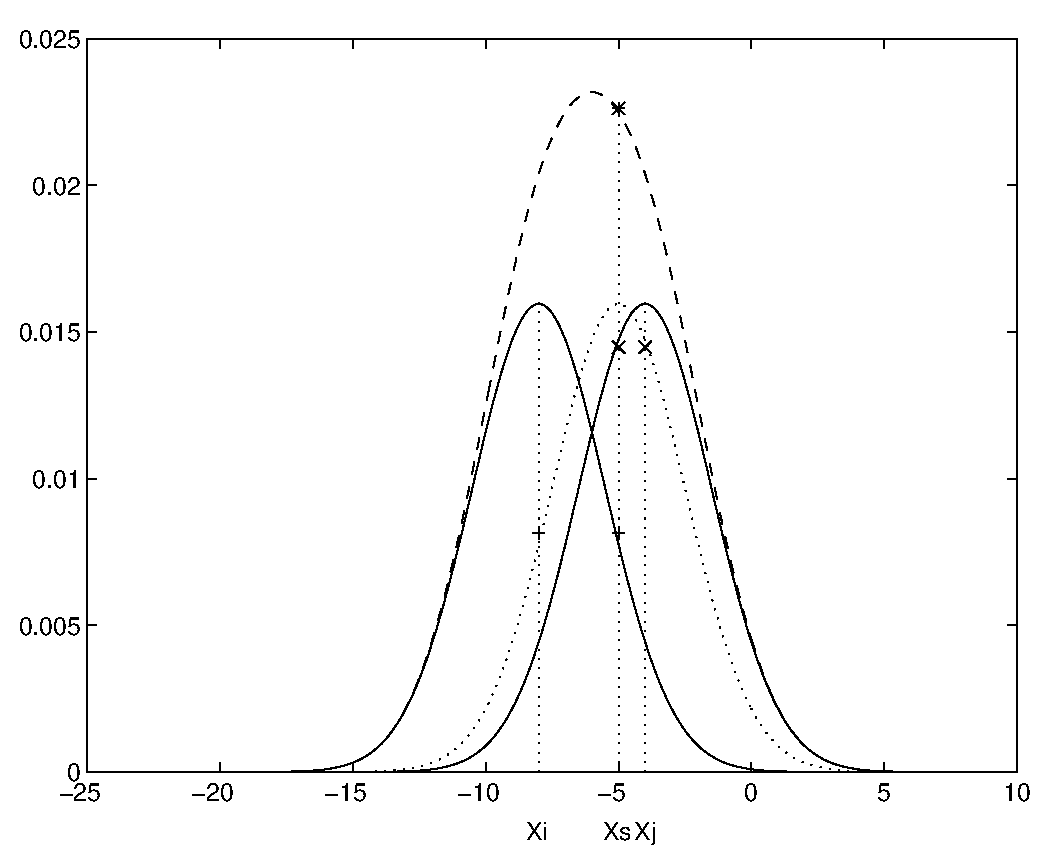
\includegraphics[height=6.2cm]{eijkel2}
% \caption{One kernel at $x_s$ (\emph{dotted kernel}) or two kernels at
% $x_i$ and $x_j$ (\textit{left and right}) lead to the same summed estimate
% at $x_s$. This shows a figure consisting of different types of
% lines. Elements of the figure described in the caption should be set in
% italics, in parentheses, as shown in this sample caption.}
% \label{fig:example}
% \end{figure}
% 
% Please define figures (and tables) as floating objects. Please avoid
% using optional location parameters like ``\verb+[h]+" for ``here".
% 
% \paragraph{Remark 1.}
% 
% In the printed volumes, illustrations are generally black and white
% (halftones), and only in exceptional cases, and if the author is
% prepared to cover the extra cost for color reproduction, are colored
% pictures accepted. Colored pictures are welcome in the electronic
% version free of charge. If you send colored figures that are to be
% printed in black and white, please make sure that they really are
% legible in black and white. Some colors as well as the contrast of
% converted colors show up very poorly when printed in black and white.
% 
% \subsection{Formulas}
% 
% Displayed equations or formulas are centered and set on a separate
% line (with an extra line or halfline space above and below). Displayed
% expressions should be numbered for reference. The numbers should be
% consecutive within each section or within the contribution,
% with numbers enclosed in parentheses and set on the right margin --
% which is the default if you use the \emph{equation} environment, e.g.,
% \begin{equation}
%   \psi (u) = \int_{o}^{T} \left[\frac{1}{2}
%   \left(\Lambda_{o}^{-1} u,u\right) + N^{\ast} (-u)\right] dt \;  .
% \end{equation}
% 
% Equations should be punctuated in the same way as ordinary
% text but with a small space before the end punctuation mark.
% 
% \subsection{Footnotes}
% 
% The superscript numeral used to refer to a footnote appears in the text
% either directly after the word to be discussed or -- in relation to a
% phrase or a sentence -- following the punctuation sign (comma,
% semicolon, or period). Footnotes should appear at the bottom of
% the
% normal text area, with a line of about 2~cm set
% immediately above them.\footnote{The footnote numeral is set flush left
% and the text follows with the usual word spacing.}
% 
% \subsection{Program Code}
% 
% Program listings or program commands in the text are normally set in
% typewriter font, e.g., CMTT10 or Courier.
% 
% \medskip
% 
% \noindent
% {\it Example of a Computer Program}
% \begin{verbatim}
% program Inflation (Output)
%   {Assuming annual inflation rates of 7%, 8%, and 10%,...
%    years};
%    const
%      MaxYears = 10;
%    var
%      Year: 0..MaxYears;
%      Factor1, Factor2, Factor3: Real;
%    begin
%      Year := 0;
%      Factor1 := 1.0; Factor2 := 1.0; Factor3 := 1.0;
%      WriteLn('Year  7% 8% 10%'); WriteLn;
%      repeat
%        Year := Year + 1;
%        Factor1 := Factor1 * 1.07;
%        Factor2 := Factor2 * 1.08;
%        Factor3 := Factor3 * 1.10;
%        WriteLn(Year:5,Factor1:7:3,Factor2:7:3,Factor3:7:3)
%      until Year = MaxYears
% end.
% \end{verbatim}
% %
% \noindent
% {\small (Example from Jensen K., Wirth N. (1991) Pascal user manual and
% report. Springer, New York)}
% 
% \subsection{Citations}
% 
% For citations in the text please use
% square brackets and consecutive numbers: \cite{jour}, \cite{lncschap},
% \cite{proceeding1} -- provided automatically
% by \LaTeX 's \verb|\cite| \dots\verb|\bibitem| mechanism.
% 
% \subsection{Page Numbering and Running Heads}
% 
% There is no need to include page numbers. If your paper title is too
% long to serve as a running head, it will be shortened. Your suggestion
% as to how to shorten it would be most welcome.
% 
% 
% \section{BibTeX Entries}
% 
% The correct BibTeX entries for the Lecture Notes in Computer Science
% volumes can be found at the following Website shortly after the
% publication of the book:
% \url{http://www.informatik.uni-trier.de/~ley/db/journals/lncs.html}
% 
% \subsubsection*{Acknowledgments.} The heading should be treated as a
% subsubsection heading and should not be assigned a number.
% 
% \section{The References Section}\label{references}
% 
% In order to permit cross referencing within LNCS-Online, and eventually
% between different publishers and their online databases, LNCS will,
% from now on, be standardizing the format of the references. This new
% feature will increase the visibility of publications and facilitate
% academic research considerably. Please base your references on the
% examples below. References that don't adhere to this style will be
% reformatted by Springer. You should therefore check your references
% thoroughly when you receive the final pdf of your paper.
% The reference section must be complete. You may not omit references.
% Instructions as to where to find a fuller version of the references are
% not permissible.
% 
% We only accept references written using the latin alphabet. If the title
% of the book you are referring to is in Russian or Chinese, then please write
% (in Russian) or (in Chinese) at the end of the transcript or translation
% of the title.
% 
% The following section shows a sample reference list with entries for
% journal articles \cite{jour}, an LNCS chapter \cite{lncschap}, a book
% \cite{book}, proceedings without editors \cite{proceeding1} and
% \cite{proceeding2}, as well as a URL \cite{url}.
% Please note that proceedings published in LNCS are not cited with their
% full titles, but with their acronyms!
% 
% \begin{thebibliography}{4}
% 
% \bibitem{jour} Smith, T.F., Waterman, M.S.: Identification of Common Molecular
% Subsequences. J. Mol. Biol. 147, 195--197 (1981)
% 
% \bibitem{lncschap} May, P., Ehrlich, H.C., Steinke, T.: ZIB Structure Prediction Pipeline:
% Composing a Complex Biological Workflow through Web Services. In: Nagel,
% W.E., Walter, W.V., Lehner, W. (eds.) Euro-Par 2006. LNCS, vol. 4128,
% pp. 1148--1158. Springer, Heidelberg (2006)
% 
% \bibitem{book} Foster, I., Kesselman, C.: The Grid: Blueprint for a New Computing
% Infrastructure. Morgan Kaufmann, San Francisco (1999)
% 
% \bibitem{proceeding1} Czajkowski, K., Fitzgerald, S., Foster, I., Kesselman, C.: Grid
% Information Services for Distributed Resource Sharing. In: 10th IEEE
% International Symposium on High Performance Distributed Computing, pp.
% 181--184. IEEE Press, New York (2001)
% 
% \bibitem{proceeding2} Foster, I., Kesselman, C., Nick, J., Tuecke, S.: The Physiology of the
% Grid: an Open Grid Services Architecture for Distributed Systems
% Integration. Technical report, Global Grid Forum (2002)
% 
% \bibitem{url} National Center for Biotechnology Information, \url{http://www.ncbi.nlm.nih.gov}
% 
% \end{thebibliography}



\end{document}
